\documentclass[multi=page, border=0.5cm]{standalone}
\usepackage{calculator}
\usepackage[svgnames]{xcolor}
\usepackage{tikz}
\usetikzlibrary{arrows, arrows.meta, positioning}

\tikzset{    
    quad1/.style={ color=red,    thin, scale = 4 },
    quad2/.style={ color=blue,   thin, scale = 3 },
    quad3/.style={ color=magenta,thin, scale = 2 }
}

\definecolor{light-gray}{gray}{0.95}

\begin{document}
\begin{page}
    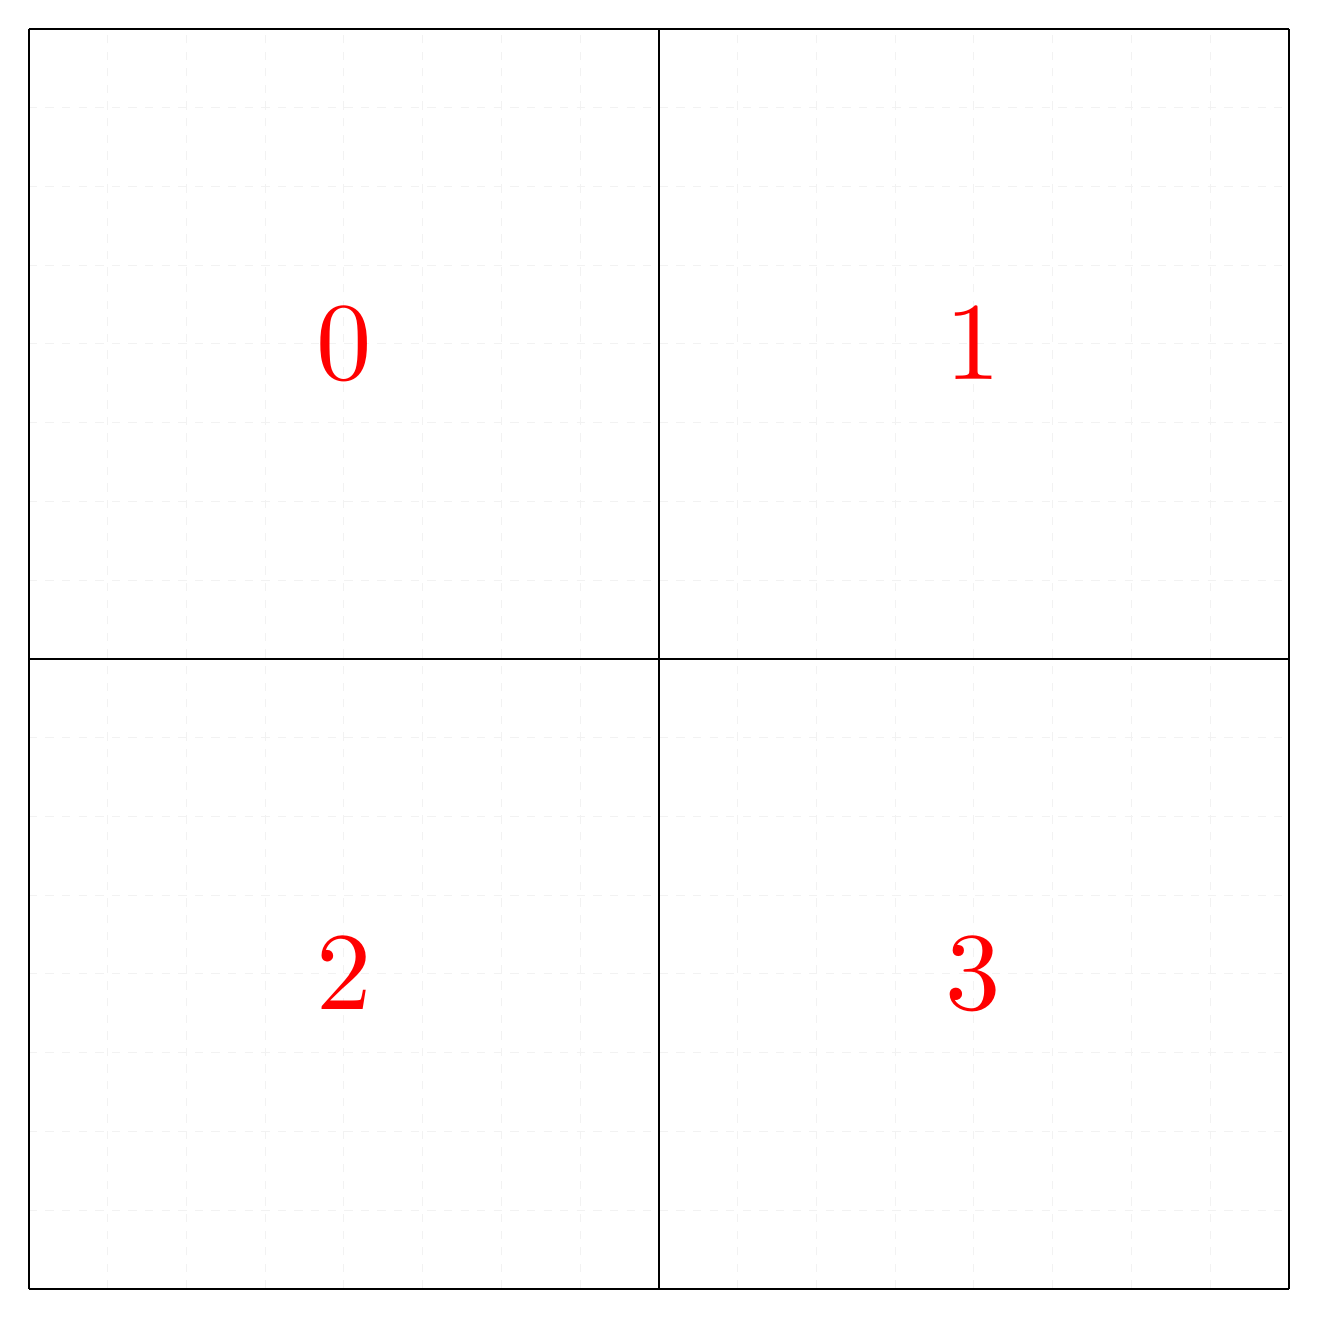
\begin{tikzpicture}
        \draw[step=1, very thin, light-gray, dashed] (0,0) grid (16,16);

        \draw[step=8, thick, black] (0,0) grid (16,16);
        \node[quad1] at (4,12)  {0};
        \node[quad1] at (12,12) {1};
        \node[quad1] at (4,4)   {2};
        \node[quad1] at (12,4)  {3};
    \end{tikzpicture}
\end{page}

\begin{page}
    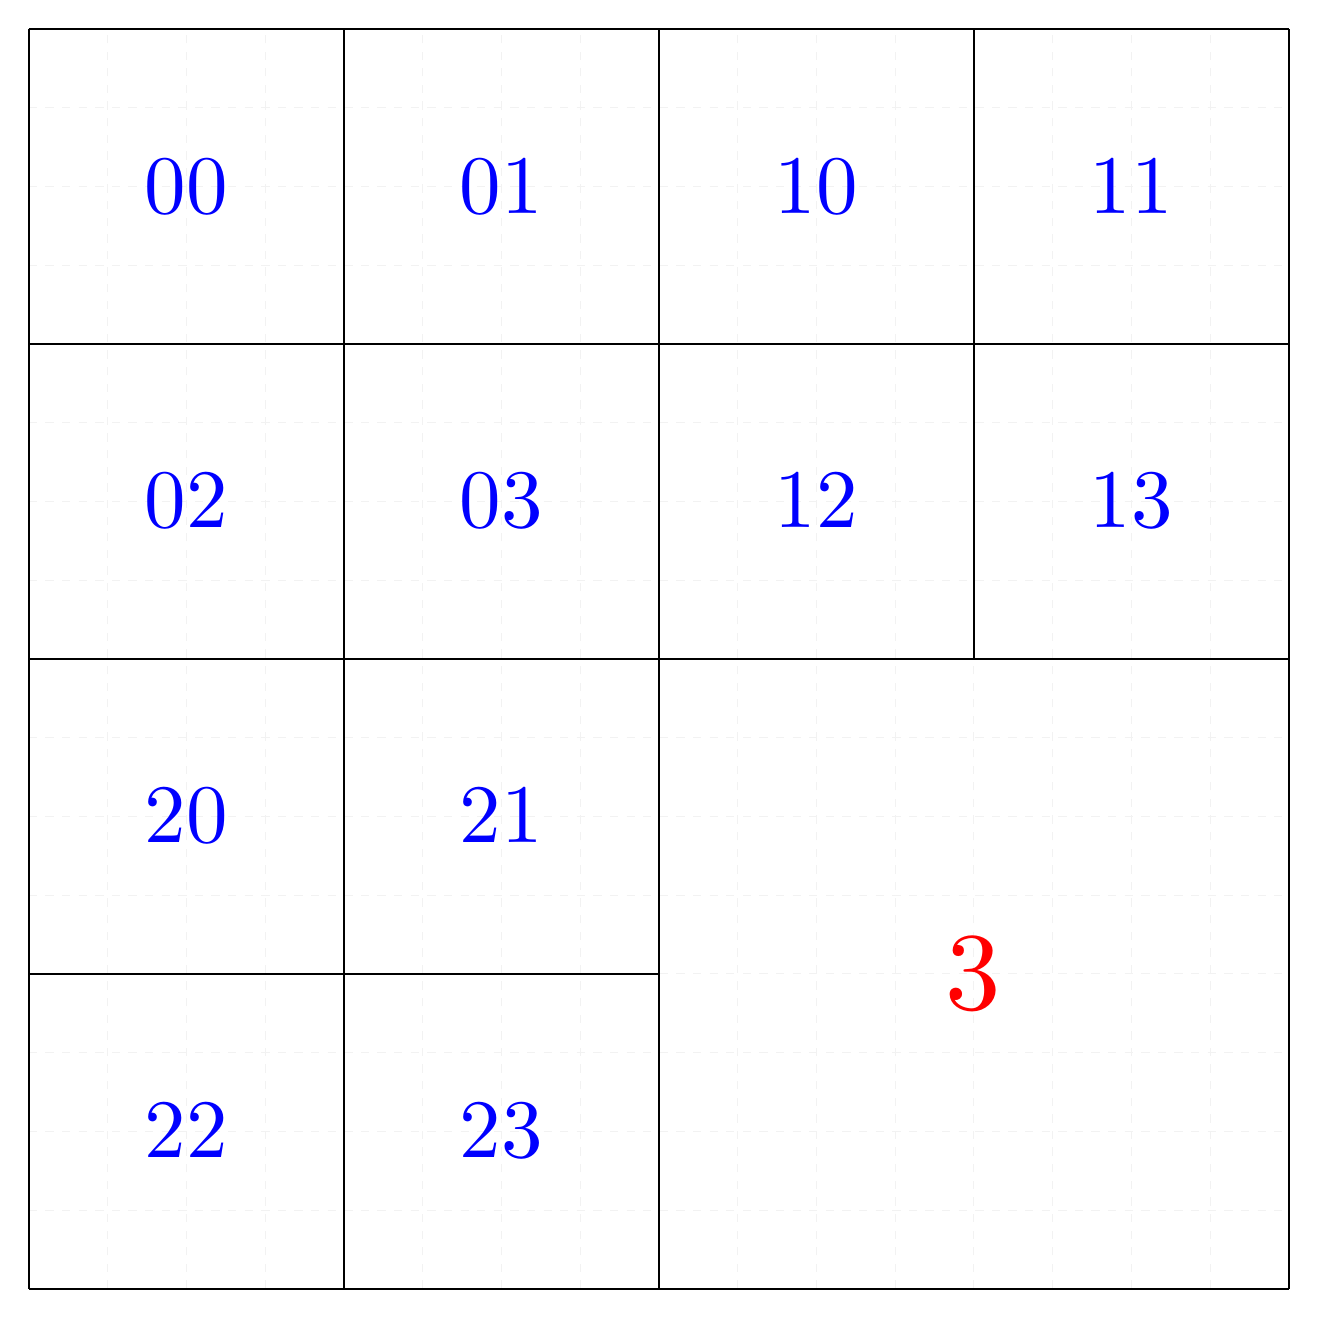
\begin{tikzpicture}
        \draw[step=1, very thin, light-gray, dashed] (0,0) grid (16,16);

        \draw[step=8, thick, black] (0,0) grid (16,16);
        \draw[step=4, thick, black] (8,8) grid (16,16);
        \draw[step=4, thick, black] (0,8) grid (8,16);
        \draw[step=4, thick, black] (0,0) grid (8,8);
        \node[quad2] at (2,14)  {00};
        \node[quad2] at (6,14)  {01};
        \node[quad2] at (2,10)  {02};
        \node[quad2] at (6,10)  {03};
        \node[quad2] at (10,14) {10};
        \node[quad2] at (14,14) {11};
        \node[quad2] at (10,10) {12};
        \node[quad2] at (14,10) {13};
        \node[quad2] at (2,6)   {20};
        \node[quad2] at (6,6)   {21};
        \node[quad2] at (2,2)   {22};
        \node[quad2] at (6,2)   {23};
        \node[quad1] at (12,4)  {3};
    \end{tikzpicture}
\end{page}

\begin{page}
    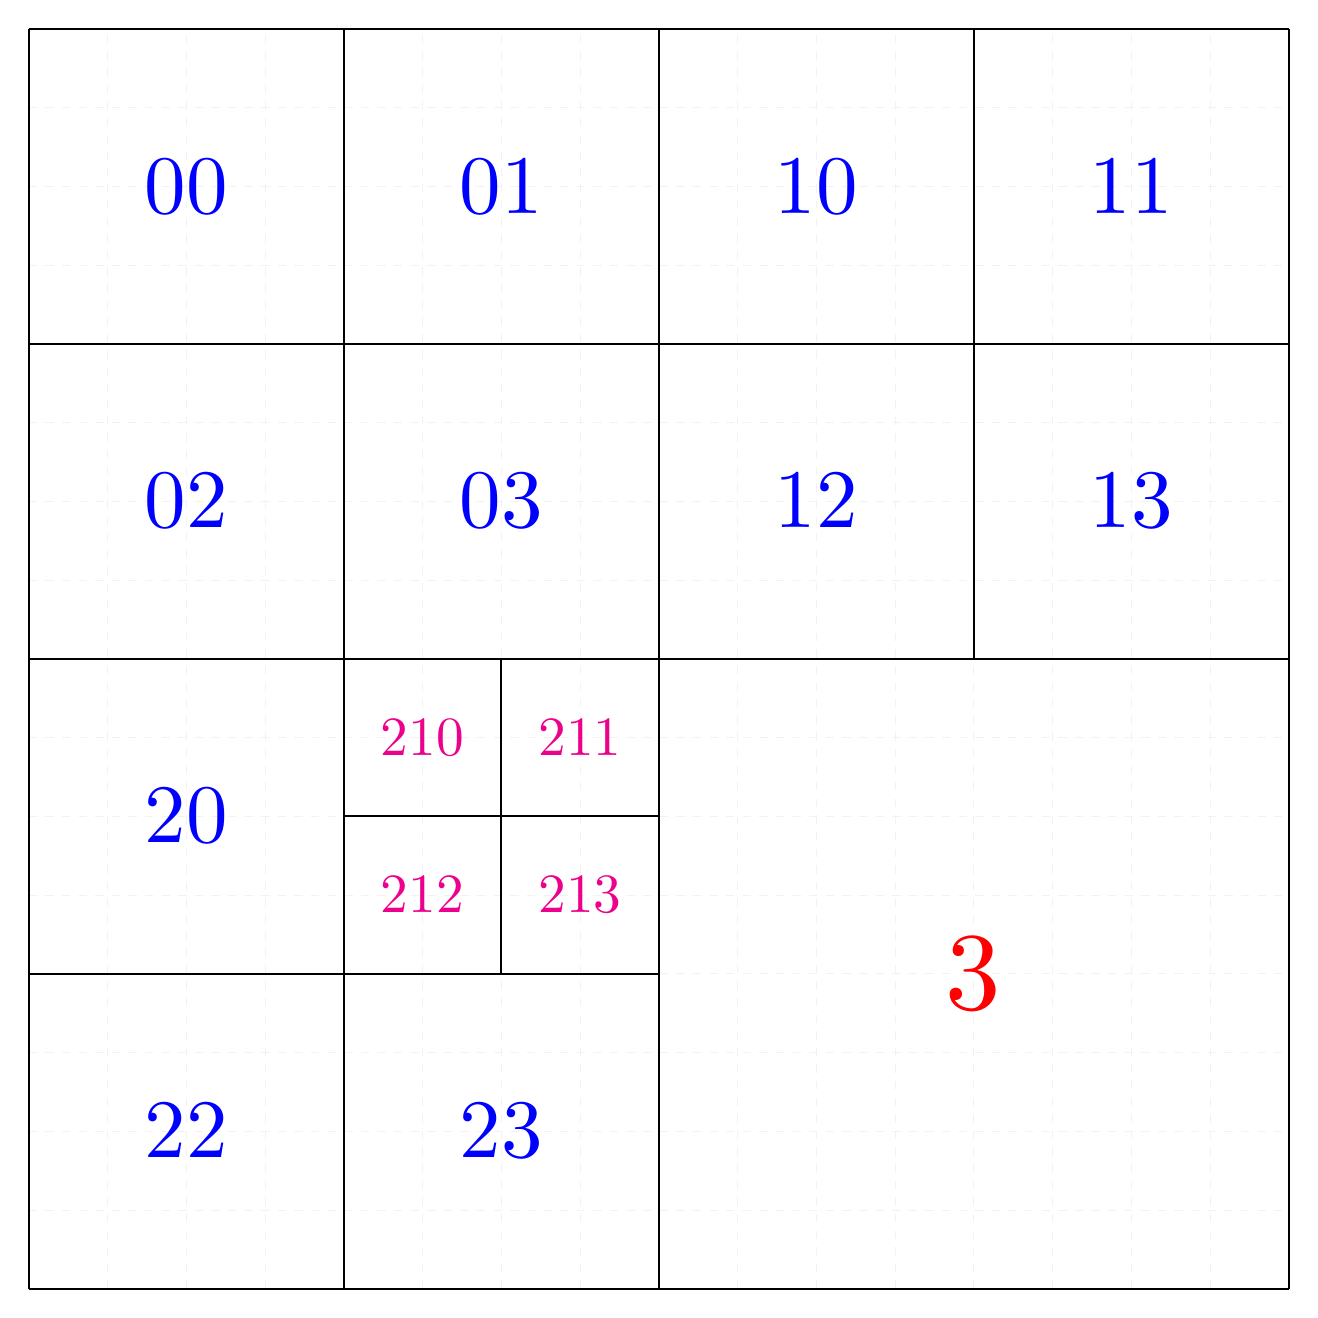
\begin{tikzpicture}
        \draw[step=1, very thin, light-gray, dashed] (0,0) grid (16,16);

        \draw[step=8, thick, black] (0,0) grid (16,16);
        \draw[step=4, thick, black] (8,8) grid (16,16);
        \draw[step=4, thick, black] (0,8) grid (8,16);
        \draw[step=4, thick, black] (0,0) grid (8,8);
        \draw[step=2, thick, black] (4,4) grid (8,8);
        \node[quad2] at (2,14)  {00};
        \node[quad2] at (6,14)  {01};
        \node[quad2] at (2,10)  {02};
        \node[quad2] at (6,10)  {03};
        \node[quad2] at (10,14) {10};
        \node[quad2] at (14,14) {11};
        \node[quad2] at (10,10) {12};
        \node[quad2] at (14,10) {13};
        \node[quad2] at (2,6)   {20};
        \node[quad3] at (5,7)   {210};
        \node[quad3] at (7,7)   {211};
        \node[quad3] at (5,5)   {212};
        \node[quad3] at (7,5)   {213};
        \node[quad2] at (2,2)   {22};
        \node[quad2] at (6,2)   {23};
        \node[quad1] at (12,4)  {3};
    \end{tikzpicture}
\end{page}
\end{document} 
